% http://guitarpenguin.is-programmer.com/posts/48869.html
% fix tex4ht:
% https://tex.stackexchange.com/questions/185349/error-using-pgfsysdriver-with-tex4ht-only-shows-up-with-texlive-2014-ok-with-t

\documentclass{article}
\def\pgfsysdriver{pgfsys-tex4ht.def}
%There is specialized output driver for use with tex4ht in Tikz. Using it, diagrams are saved in SVG.
\usepackage{tikz}
\usepackage{pgf}

\usetikzlibrary{automata}
\usetikzlibrary{positioning,chains,fit,shapes,calc}
\usetikzlibrary{arrows,shadows,trees}

\begin{document}
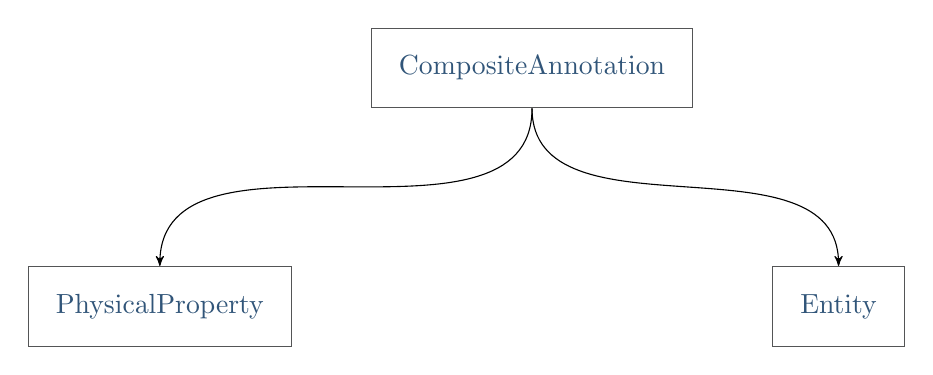
\begin{tikzpicture}[->,>=stealth',node distance=1cm]

  \tikzstyle{block}=[fill=white, draw={rgb:red,225;green,228;blue,229}, text={rgb:red,64;green,112;blue,160}, scale=1.0, inner sep=10pt]
  \node[block] (CompositeAnnotation) at (10,0) {CompositeAnnotation};
  \node[block,below left = 2cm and 1cm of CompositeAnnotation] (PhysicalProperty) {PhysicalProperty};
  \node[block,below right = 2cm and 1cm of CompositeAnnotation] (Entity) {Entity};
  \draw (CompositeAnnotation.south) to [out=-90,in=90] (PhysicalProperty.north);
  \draw (CompositeAnnotation.south) to [out=-90,in=90] (Entity.north);

\end{tikzpicture}
\end{document}
